Finite element analysis (FEA) is highly effective at calculating stress intensity factors (SIFs) for cracks in arbitrary geometries. However, despite its accuracy, FEA has notable limitations. One significant drawback is its demanding computational requirements, as well as the need for a skilled analyst to achieve reliable results. These factors can lead to substantial time and resource investments, especially when numerous calculations are required, such as those for fatigue and uncertainty assessment. To address these challenges, many engineers in industry often rely on handbook solutions. These solutions offer a practical way to estimate SIFs for common, simplified crack scenarios, and when applied correctly, they can yield very accurate results. Additionally, they entail significantly reduced computational costs compared to FEA.


The Raju Newman equations are widely used set of handbook equations that provide predictions for SIFs under various crack shapes and loading conditions \cite{RNeqnsbook}. These handbook solutions are user-friendly, given their straightforward polynomial forms. However, their ease of use sometimes leads to their application in situations that do not align with the assumptions and limitations of the original idealized model, resulting in inaccurate predictions. This research specifically focuses on the case of a semi-elliptical surface crack in a finite plate subjected to mode I tension. Raju and Newman have an equation designed for this particular crack scenario. Since the introduction of the Raju Newman equations for a semi-elliptical surface cracks alternative models have been proposed that allow for more complex loading conditions such as the models created by \cite{Wang1995, Pommier1999}. The model created by Wang and Lambert allows for linear stress functions \cite{Wang1995}. Pommier, et al. created a model that could predict SIFs under polynomial stress fields \cite{Pommier1999}.

 To prevent the improper use of SIF equations, it is crucial to build a more extensive database of SIF solutions. Machine learning (ML) can play a pivotal role in automating the creation of these SIF solutions. ML enables the development of models for more complex crack scenarios, going beyond the scope of current handbook solutions, which primarily cover idealized cases. Notably, ML has been successfully employed to produce highly accurate SIF solutions, as documented in studies such as in \cite{Zhang2023, Sobotka2022, Keprate2017, Xu2022, Seghier2020}. The advantage of ML over other techniques, like those found in \cite{RNeqnsbook, Pommier1999, Wang1995}, is its ability to be trained relatively quickly, resulting in very accurate models. This, in turn, facilitates the creation of more surrogate models. However, it's worth noting that many commonly used ML algorithms generate "black-box" models, which lack interpretability. In engineering, interpretability is crucial because engineers need to trust and explain their designs, which black-box models do not readily allow. This is why handbook solutions, such as those in \cite{RNeqnsbook}, continue to be used since they inherently offer interpretability.

This paper specifically studies the case of a semi-elliptical surface crack in a finite plate subjected to mode I tension, a common crack found in pressure vessels. An existing handbook solution by \cite{RNeqnsbook} covers this case. However, more accurate models have been developed using machine learning (ML) techniques, as demonstrated by \cite{Keprate2017, Xu2022, Seghier2020}. These ML models, utilizing methods like Gaussian processes regression and neural networks, offer higher accuracy but produce less interpretable "black-box" models. Notably, the ML models mentioned could predict SIFs at only a single point along the crack front, whereas the Raju-Newman equations can estimate SIFs across the entire crack length.

While ML models provide improved predictive capabilities, their lack of interpretability can be a drawback in certain contexts, especially when it comes to explaining and trusting the predicted SIF. The interpretability of the Raju and Newman equations gives engineers a clear understanding of how SIFs are derived, aiding decision-making and instilling confidence in the results. These equations systematically break down the crack case into subfunctions, each contributing differently to the final SIF predition. For instance, in the case of the semi-elliptical crack, they modify the analytical solution to the embedded ellipse with boundary correction functions, enhancing the inherent explainability of an analytical solution.

This research will utilize an interpretable machine learning code Bingo, developed by researchers at NASA and the University of Utah \cite{Randall2022}. Bingo generates closed-form mathematical expressions to predict SIFs along the entire crack length, offering improved accuracy and simplicity compared to the Raju-Newman equations while preserving interpretability. Thanks to the closed-form nature of Bingo's models, they can be easily integrated into existing Linear Elastic Fracture Mechanics (LEFM) software applications like NASGRO, AFGROW, and SMART|DT \cite{nasgro, afgrow, smartdt}. Closed form solutions can also be inverted to solve for applied stress for use in a constant SIF test.

\subsection{Background}
In linear elastic fracture mechanics (LEFM), the precise solution for the Stress Intensity Factor (SIF) along an elliptical crack in an infinite volume is given by the equation:

\begin{equation} \label{eqn:K_embedded_ellipse}
    K_{ee} = \sigma \frac{\sqrt{\pi a}}{E} \left( \sin^2 \phi + \frac{a^2}{c^2} \cos^2 \phi \right)^{1/4}, \text{where } a \le c, 
\end{equation}

where $a$ represents the length of the minor axis of the ellipse, $c$ represents the length of the major axis, $\sigma$ is the far-field stress, and $E$ is the complete elliptic integral of the second kind. This expression is only valid when $a \leq c$. In the context of a semi-elliptical surface crack, the values of $a$ and $c$ differ from the minor and major axes, instead representing the crack depth and half-crack surface length, respectively, as illustrated in figure \ref{fig:crack_params} \cite{tada1985}. To accommodate cases where $a/c$ will exceed 1, Raju and Newman employed a modified version of equation \ref{eqn:K_embedded_ellipse}. This modification, detailed in equation \ref{eqn:fphi}, allows for the use of all values of $a/c$.
\begin{figure}%
    \centering
    \subfloat[\centering Crack dimensions]{{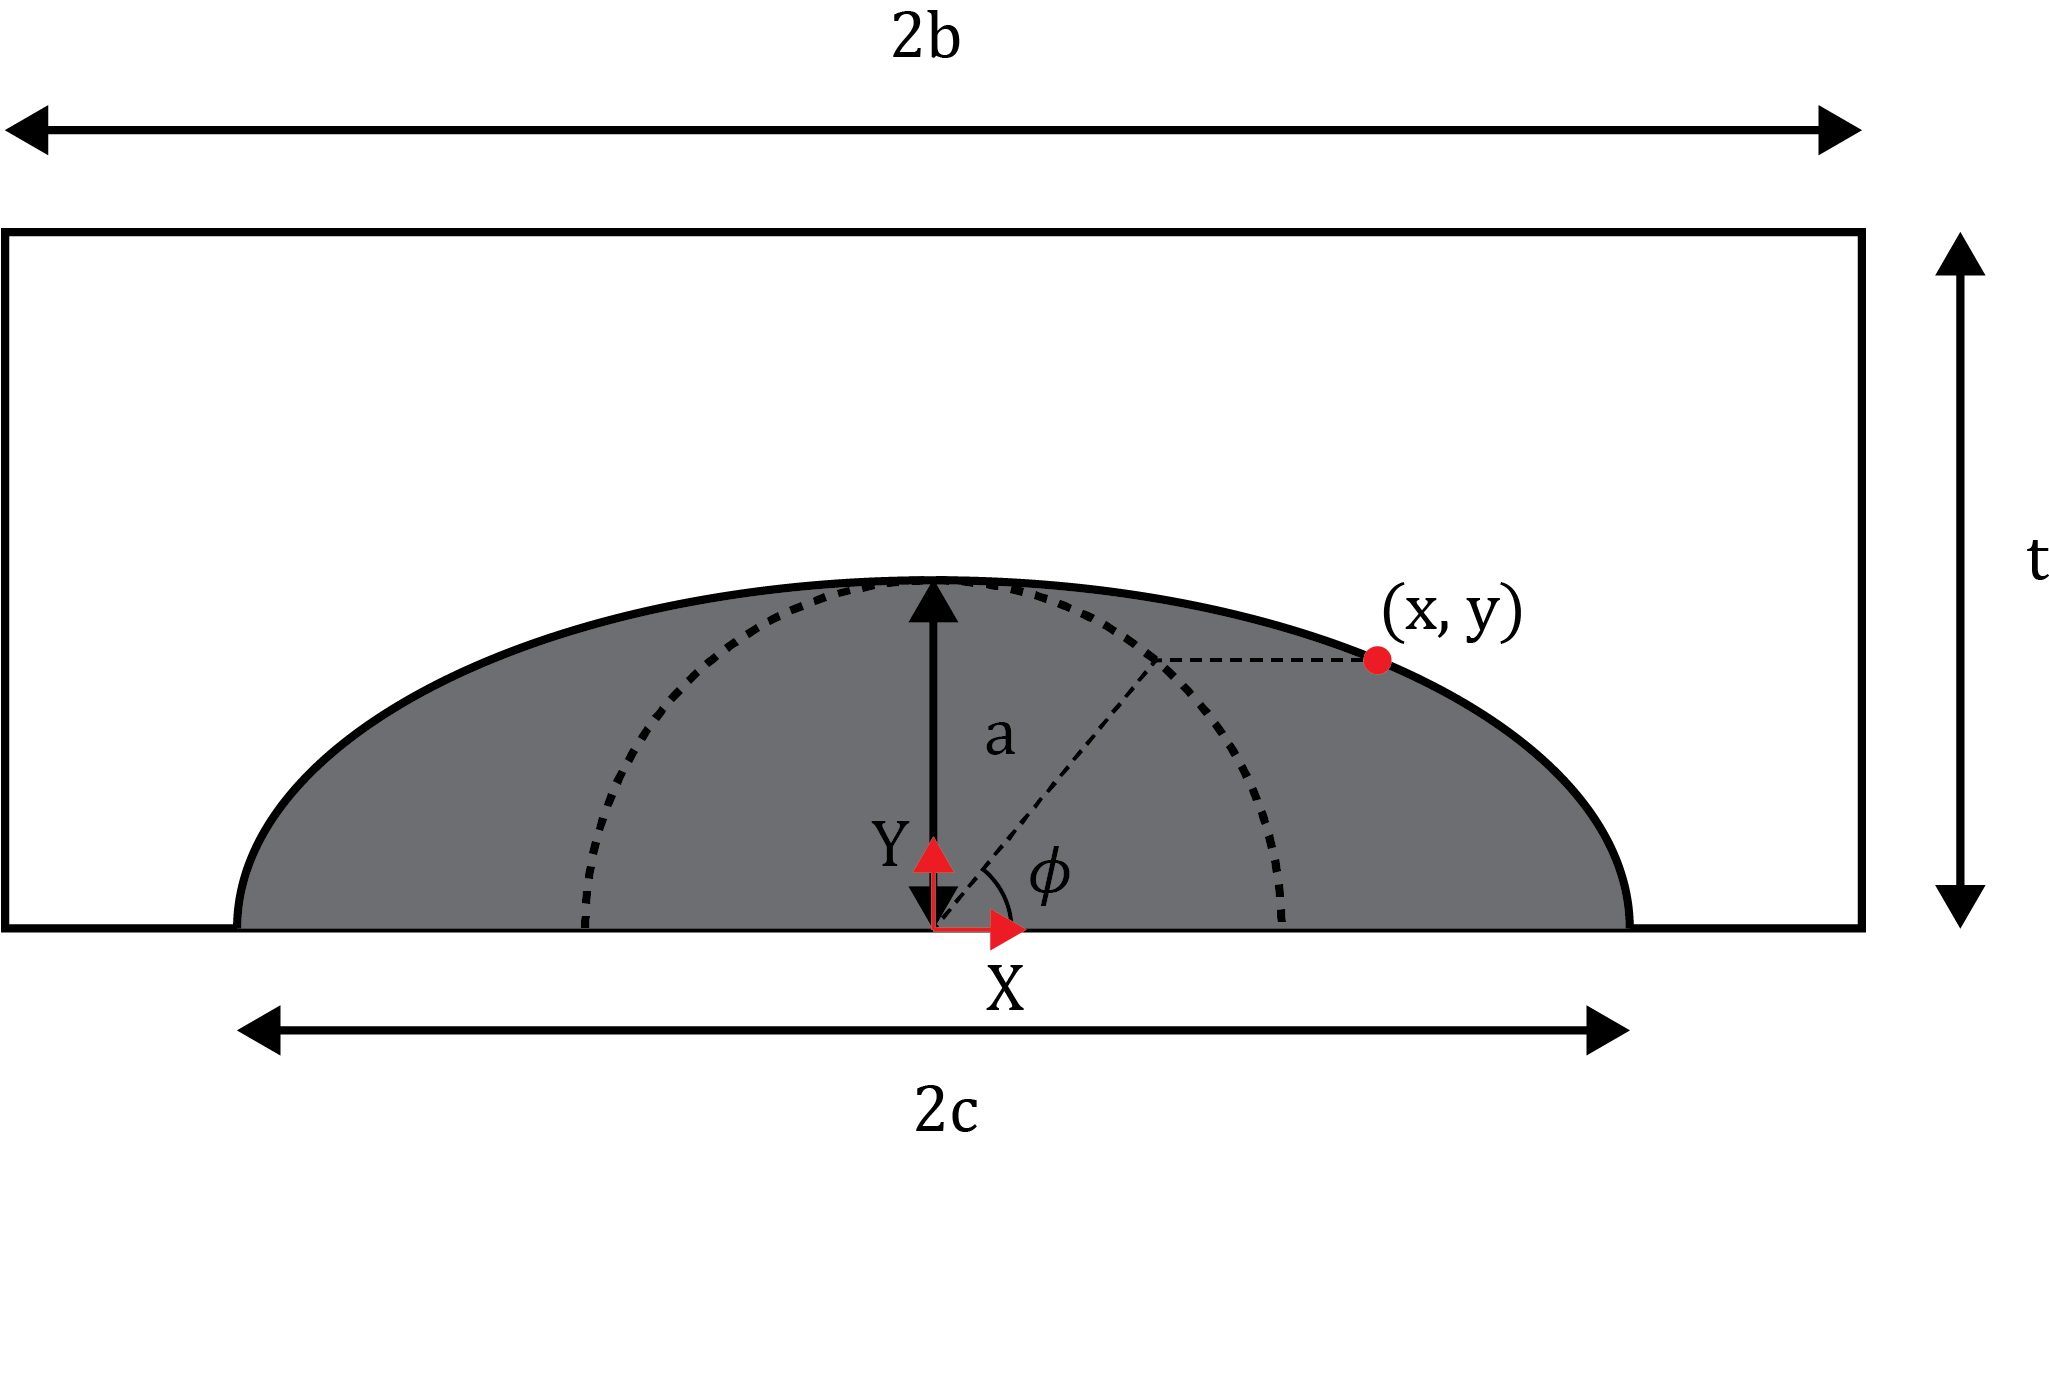
\includegraphics[width=0.5\textwidth]{geometry_figures/params.png} }}%
    \qquad
    \subfloat[\centering Ellipse dimensions]{{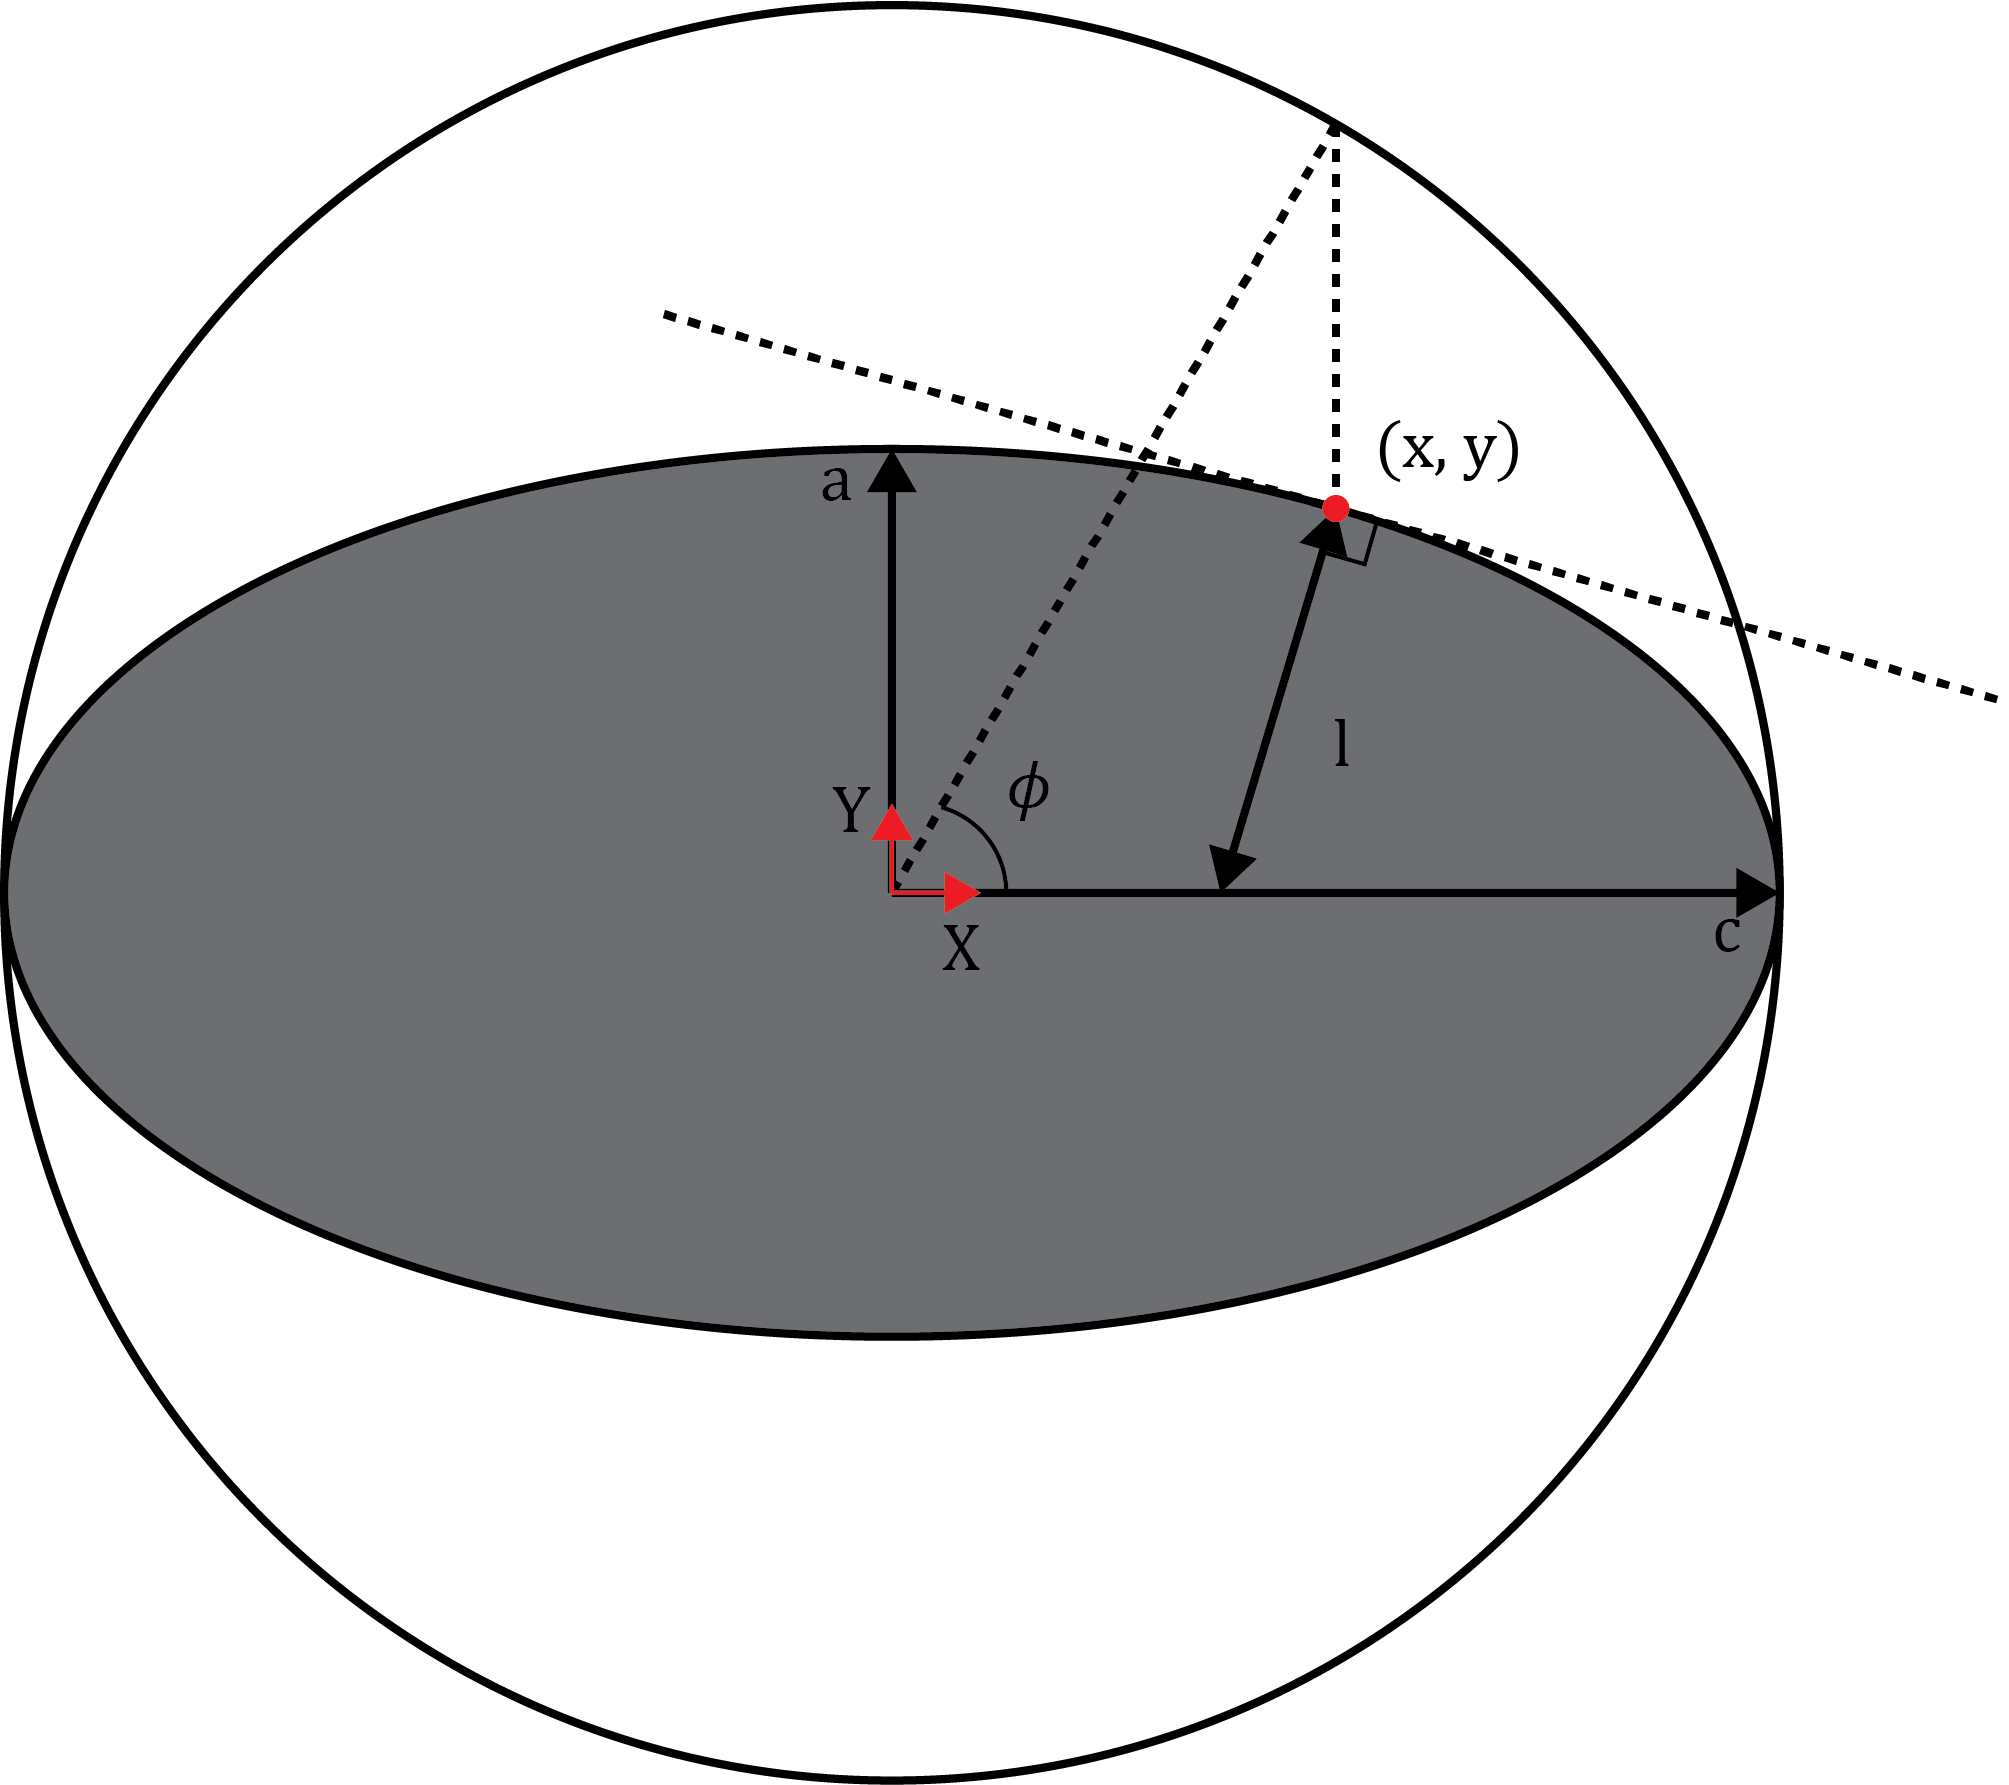
\includegraphics[width=0.5\textwidth]{geometry_figures/Ellipse.png} }}%
    \caption{(a) Crack parameters with $a$ being the crack depth and $2c$ being the surface crack length. (b) $\phi$ is defined by the angle to the inscribed circle projected to the ellipse. $l$ is defined as the distance perpendicular to the tangent line from the point of interest to the nearest axis.}%
    \label{fig:crack_params}%
\end{figure}
\begin{equation} \label{eqn:fphi}
f_{\phi} = \begin{cases}
      \left[\left(\frac{a}{c}\right)^2 \cos^2\phi + \sin^2\phi\right]^{1/4} & \text{if } \frac{a}{c} \le 1 \\
      \\
      \left[\cos^2\phi + \left(\frac{c}{a}\right)^2\sin^2\phi\right]^{1/4} & \text{if } \frac{a}{c} > 1,
    \end{cases}
\end{equation}
 which is piece-wise, resulting in equation \ref{eqn:K_embedded_ellipse_fphi}

\begin{equation} \label{eqn:K_embedded_ellipse_fphi}
    K_{ee} = \sigma \frac{\sqrt{\pi a}}{E} f_{\phi}.
\end{equation}

Equation \ref{eqn:K_embedded_ellipse_fphi} is identical to equation \ref{eqn:K_embedded_ellipse} when $a/c \le 1$. Using equation \ref{eqn:K_embedded_ellipse_fphi} and multiplying by the correction factors $f_w$, $M$, and $g$ Raju and Newman found equation \ref{eqn:RN_K}
 \begin{equation} \label{eqn:RN_K}
     K = \frac{\sqrt{\pi a}}{E} f_{\phi} f_w M g,
 \end{equation} 

which is able to predict SIFs along the length of semi-elliptical surface crack in a finite plate.

The finite width correction factor $f_w$, defined in equation \ref{eqn:RN_fw}
\begin{equation} \label{eqn:RN_fw}
    f_w = \sqrt{\sec\left(\frac{\pi c}{2b}\sqrt{\frac{a}{t}}\right)},
\end{equation}
 is a 3D extension for the equation developed in \cite{brown1966}. The finite width correction factor accounts for the finite width and thickness of the plate when $a/c = 1$ and $\phi = \pi/2$. The thickness of the plate is denoted as $t$ and the half-width of the plate is denoted as $b$ \ref{fig:crack_params}. The function $M$ accounts for changes is SIF due to the aspect ratio of the crack at the point along the crack where $\phi = \pi/2$ and is given by \ref{eqn:RN_M}
\begin{equation} \label{eqn:RN_M}
    M = M_1 + M_2\left(\frac{a}{t}\right)^2 + M_3\left(\frac{a}{t}\right)^4
\end{equation}
\begin{equation} \label{eqn:RN_M1}
    M_1 = \begin{cases}
    1.13 - 0.09\left(\frac{a}{c}\right) & \text{if } \frac{a}{c} \le 1 \\
    \\
    \sqrt{\frac{c}{a}}\left(1 + 0.04\frac{c}{a}\right) & \text{if } \frac{a}{c} > 1
    \end{cases}
\end{equation}
\begin{equation} \label{eqn:RN_M2}
    M_2 = \begin{cases}
    -0.54 + \frac{0.89}{0.2+\left(\frac{a}{c}\right)} & \text{if } \frac{a}{c} \le 1 \\
    \\
    0.2\left(\frac{c}{a}\right)^4 & \text{if } \frac{a}{c} > 1
    \end{cases}
\end{equation}
\begin{equation} \label{eqn:RN_M3}
    M_3 = \begin{cases}
    0.5 - \frac{1}{0.65+\frac{a}{c}} + 14\left(1-\frac{a}{c}\right)^{24} & \text{if } \frac{a}{c} \le 1 \\
    \\
    -0.11\left(\frac{c}{a}\right)^4 & \text{if } \frac{a}{c} > 1.
    \end{cases}
\end{equation}
The function g corrects for free surface effects and is denoted by equation \ref{eqn:RN_g}
\begin{equation} \label{eqn:RN_g}
    g = \begin{cases}
    1 + \left[0.1 + 0.35\left(\frac{a}{t}\right)^2\right]\left(1 - \sin\phi\right)^2 & \text{if } \frac{a}{c} \le 1 \\
    \\
    1 + \left[0.1 + 0.35\left(\frac{c}{a}\right)\left(\frac{a}{t}\right)^2\right]\left(1 - \sin\phi\right) & \text{if } \frac{a}{c} > 1.
    \end{cases}
\end{equation}
The function $g$ is sinusoidal, having a value of 1 at $\phi = \pi/2$.  By using this methodical approach of breaking down the problem into sub-functions that each account for a different aspect of the crack, allowed Raju and Newman to develop accurate equations that build upon the explainablity from the analytical solution of the embedded ellipse. 
